%Here is the method used to examine the question
In this chapter, the methods employed to answer the proposed question are presented. This chapter begins by establishing the task, data sets and data processing utilized in this project. Thereafter, the experimental setup is described and relevant neural network architectures are outlined. Finally, the approaches for training the generative models are presented. Three approaches of this kind have been employed in this project: standard \acrshort{vaes}, progressive \acrshort{gans} and Autoencoding \acrshort{gans}. They are presented in their respective section. 

The level of details presented here should suffice for re-implementing the algorithms and reproduce the experiments of this project. Though there exist questions which need more details to answer than what can possibly be captured in a report like this. For this purpose, the original implementation is available online\footnote{The code is availabel at: \url{www.github.com/netrome/DeepGeneration}}.

\section{Pupil Localization}
To investigate the extent to which deep generative models can act as a drop-in replacement for real data sets, a case study of Pupil Localization was performed. Pupil Localization is an instance of the problem of object Localization. The objective is to localize the pupil in an image of an eye. In normal cases, pupil localization is not achieved with deep neural networks. There already exist more computationally efficient methods for this task, such as the method proposed in \parencite{markuvs2014eye}. On the other hand deep neural networks for semantic segmentation are capable of predicting high quality segmentation maps on diverse complicated data sets \parencite{ChenPK0Y16semantic} and should therefore perform extraordinary well on the relatively simple task of pupil localization.

By comparing pupil localization performance when the localizer is trained on either data from a deep generative model or data from the original data set and tested on data from either of the domains, the usability of the generated data for model training or evaluation can be assessed. Especially the case of training on generated data and testing on the original data is interesting. Assuming that the localizer learns the optimal mapping for the data domain it is trained on, the performance of this localizer can then be used as a measure of the quality and usability of the generated data. 

The benefit of this approach is that the cross-data localization error can easily be compared to the intra-data localization error . The relative magnitutes of these losses indicate the difficulties of adapting models between the domains. This enables not only giving a binary answer to the original question of this project but showing how close to succeeding the tested methods are in learning the data distribution.

\section{Synthetic Data}
The initial experiments in this study are performed on synthetic data obtained through rendering of a 3D head model in a data generation framework. This framework is based on the work of \textcite{swirski2014rendering} and utilizes the same head rig. Two data sets with resolution 256x256 was generated, a training set consisting of 3000 images and a test set with 300 images. For reproducability, these data sets will become publicly available at the time of publication.

The synthetic data sets are fully annotated with automatically generated ground truth labels. The relevant labels for the experiments are converted to heatmaps when loaded for training and evaluation as in most cases of semantic segmentation \parencite{guo2017review}. These heatmaps are thereafter concatenated with the real images, forming feature maps of shape 2x320x320. By viewing the annotations as a part of the data, unsupervised models that learn the data distribution implicitly learn the relations between the annotations and the images.

\section{Real World Data}
A propiretary data set was used to further evaluate the methods. The data set consits of 9605 different manually annotated recordings of human subjects looking at a screen, split into a training set of 1000 recordings and a test set of 8605 recordings. Each recording consists of a set of ROI images of the eye region of the subjects. 

To adapt this data to the Pupil Regression framework, the images were cropped to 256x256 patches around the eyes. The cropping was random to ensure that the pupil is not always centered in the image, which otherwise could cause the networks to learn undesired patterns such as always producing a trivial prediction in the center of the image. 

During data sampling, the probabilites of the individual images were weighted in such a way that the separate recordings were equally probable to appear. This prevents recordings with more images to be over-representative during training, which otherwise could cause the models to over-adjust to the conditions of these recordings.

\section{Network architectures}
The deep generative models as well as the Pupil Localizer are based on deep convolutional neural networks. There are four different types of networks that are utilized in the different models in this work: Generators, discriminators, encoders and transformers. 

The default generator architecture is outlined in table \ref{tab:generator}. The default discriminator architecture is outlined in table \ref{tab:discriminator}. The main structure of these networks follows the architectures used by \textcite{karras2017progressive}, however the feature maps and instead of using non-parametric upsampling followed by an extra convolution the upsampling is performed with fractionally strided convolutions. These changes are motivated by the limited time-frame of this project as they enable faster training of the networks. Furthermore the data sets of this project are believed to be of less complexity than those of \textcite{karras2017progressive}, whereby less parameters should be necessary in the networks.

The encoder follows the structure of the discriminator but does not use minibatch discrimination, and the output shape is adjusted to the size of the latent space. 

The transformer is only used for Pupil Localization and is a normal image-to-image network. The structure of the transformer is shown in table \ref{tab:transformer}.

%...relevant network architectures are described here, together with figures and stuff. Base it around GAN networks, the small differences in the encoders can be explained afterwards.

\begin{table}[t]
    \centering
    \caption{Generator architecture used in the experiments. Feature normalization and leaky ReLUs were applied after each convolution except the last one.}
    \label{tab:generator}
    \begin{tabular}{|lll|}
        \hline
        %\multicolumn{3}{c}{Generator}           \\ 
        Operation          & Output shape     & Stride \\ \hline
        Input              & 128x1x1   & 1      \\
        Conv 4x4           & 128x4x4   & 1      \\
        Conv 3x3           & 128x4x4   & 1      \\ \hline
        Transpose Conv 2x2 & 128x8x8   & 2      \\
        Conv 3x3           & 112x8x8   & 1      \\ \hline
        Transpose Conv 2x2 & 11216x16   & 2      \\
        Conv 3x3           & 96x16x16   & 1      \\ \hline
        Transpose Conv 2x2 & 96x32x32   & 2      \\
        Conv 3x3           & 80x32x32   & 1      \\ \hline
        Transpose Conv 2x2 & 80x64x64   & 2      \\
        Conv 3x3           & 64x64x64   & 1      \\ \hline
        Transpose Conv 2x2 & 64x128x128   & 2      \\
        Conv 3x3           & 32x128x128   & 1      \\ \hline
        Transpose Conv 2x2 & 32x256x256   & 2      \\
        Conv 3x3           & 16x256x256   & 1      \\ \hline
        Conv 1x1           & 2x256x256 & 1        \\ \hline
    \end{tabular}
\end{table}

\begin{table}[t]
    \centering
    \caption{Discriminator architecture, Leaky ReLUs were applied after each convolution except the last one.}
    \label{tab:discriminator}
    \begin{tabular}{|lll|}
        \hline
        %\multicolumn{3}{c}{Discriminator}           \\ 
        Operation          & Output shape     & Stride \\ \hline
        Input              & 2x256x256   & 1   \\
        Conv 1x1           & 16x256x256 & 1    \\ 
        Conv 3x3           & 32x256x256 & 1    \\ 
        Conv 2x2           & 32x128x128 & 2    \\ \hline
        Conv 3x3           & 64x128x128 & 1    \\ 
        Conv 2x2           & 64x64x64 & 2      \\ \hline
        Conv 3x3           & 80x64x64 & 1      \\ 
        Conv 2x2           & 80x32x32 & 2      \\ \hline
        Conv 3x3           & 96x32x32 & 1      \\ 
        Conv 2x2           & 96x16x16 & 2      \\ \hline
        Conv 3x3           & 112x16x16 & 1     \\ 
        Conv 2x2           & 112x8x8 & 2       \\ \hline
        Conv 3x3           & 128x8x8 & 1       \\ 
        Conv 2x2           & 128x4x4 & 2       \\ \hline
        Minibatch stddev
        Conv 3x3           & 128x4x4   & 1     \\
        Conv 4x4           & 128x1x1   & 1     \\ 
        Fully connected    & 1x1 & 1         \\ \hline
    \end{tabular}
\end{table}

\begin{table}[t]
    \centering
    \caption{Transformer architecture used in the experiments. Skip layers were introduced as indicated in the table. Leaky ReLUs were applied after each convolution except the last one. In the prescence of skip connections the addition of the feature maps was performed before the Leaky ReLUs were applied.}
    \label{tab:transformer}
    \begin{tabular}{|lll|}
        \hline
        %\multicolumn{3}{c}{Generator}           \\ 
        Operation           & Output shape  & Stride \\ \hline
        Input               & 1x256x256     & 1     \\
        Conv 1x1 (1)           & 16x256x256    & 1     \\
        Conv 3x3 (2)            & 32x128x128    & 2     \\    
        Conv 3x3 (3)           & 64x64x64    & 2     \\ 
        Conv 3x3 (4)           & 128x32x32    & 2    \\ 
        Conv 3x3 (5)           & 256x16x16    & 2    \\ 
        Conv 3x3 (6)           & 256x8x8     & 2    \\ 
        Conv 3x3            & 256x4x4    & 2    \\ \hline
        Transpose Conv 4x4 + (6)  & 256x8x8    & 2    \\
        Transpose Conv 4x4 + (5) & 256x16x16    & 2    \\
        Transpose Conv 4x4 + (4) & 128x32x32    & 2    \\
        Transpose Conv 4x4 + (3) & 64x64x64    & 2    \\
        Transpose Conv 4x4 + (2) & 32x128x128    & 2    \\
        Transpose Conv 4x4 + (1)  & 16x256x256    & 2    \\
        Conv 1x1            & 1x256x256    & 1     \\ \hline
    \end{tabular}
\end{table}

\section{\acrlong{vaes}}
A \acrlong{vae} was constructed and trained on the synthetic data as a baseline for further experiments. The advantages of using \acrshort{vaes} for data generation in contrast to \acrshort{gans} is that they are easier to train and does not suffer from vanishing modes of data.

The \acrlong{vae} was designed using the default generator network as a decoder and the default encoder network with an output shape of 128x2. In this framework, the encoder output is interpreted as the mean values and the standard deviations of a 128-dimensional isotropic gaussian distribution. Using $E$ to denote the encoder function, this can be formulated as $P(Z|X=x) \in \mathcal{N}(\mu, \sigma)$, where $(\mu, \sigma) = E(x)$. Furthermore, the posterior $P(X|Z=z)$ is modelled as a Laplace distribution where the mean value is the generator output as $P(X|Z=z) \in \text{Laplace}(G(z), b)$, where $b$ is taken to be a hyperparameter.

\section{\acrlong{wgan}}
The \acrfull{wgan} was adopted as a second baseline to compare against more complex methods. It was chosen because it currently is one of the most prominent \acrshort{gan} variations. Furthermore the progressive \acrshort{gan} of next section is based on the \acrshort{wgan} causing it to be a natural baseline. 

The \acrshort{wgan} was constructed using the default generator and discriminator. To enforce the discriminator to be Lipschitz 1, gradient penalty was used as described in \parencite{gulrajani2017improved}.

\section{Progressive \acrshort{gan}}
The most advanced method tested in this project was the progressive \acrshort{gan}, proposed by \textcite{karras2017progressive}. The proposed advantages of this approach over other existing \acrshort{gan} variations is two-fold. Firstly, there is reason to believe that the quality and diversity of the generated samples are improved by the progressive training. Secondly, the training stability is believed to increase. However due to the novelty of the approach and the lack of extensive evaluations of different \acrshort{gans} it is difficult to know for sure if this is the case.

The progressive \acrshort{gan} was adopted because of the proposed training stability that arises from progressivly increasing the complexity of the learned task. It was implemented using the default generator and discriminator. The training was divided in six stages, each stage producing images with four times the resoulution of the previous stage. As in the original article, each stage contained an extra 1x1 convolution to produce 2-channel images. The illustrated networks are therefore examples of stage-6 networks. To obtain a stage-5 network one should simply reshape the 1x1 convolutions and remove the two last (non 1x1) convolutions of the generator and the two first (non 1x1) convolutions of the generator.

As in the original article, feature normalization, minibatch discrimination and smooth fade-in of new layers was implemented as closely as possible to the original formulation.

%\subsection{Freeze in new layers}
%\begin{figure}[t]
%    \centering
%    \begin{subfigure}[b]{0.45\textwidth}
%        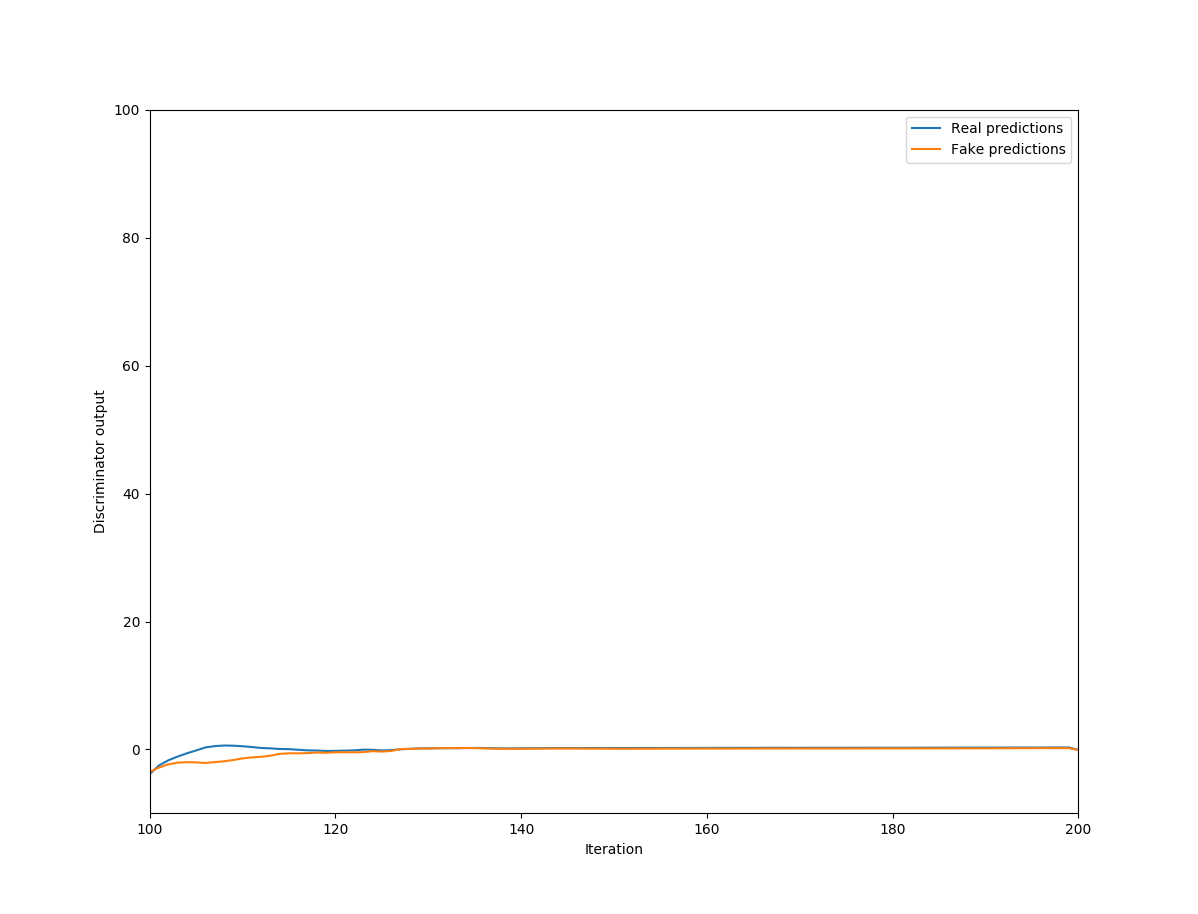
\includegraphics[width=\textwidth]{results/freezeInDG1.png}
%        \caption{Weight freezing in old layers}
%        \label{fig:freezeInDG1}
%    \end{subfigure}
%    \begin{subfigure}[b]{0.45\textwidth}
%        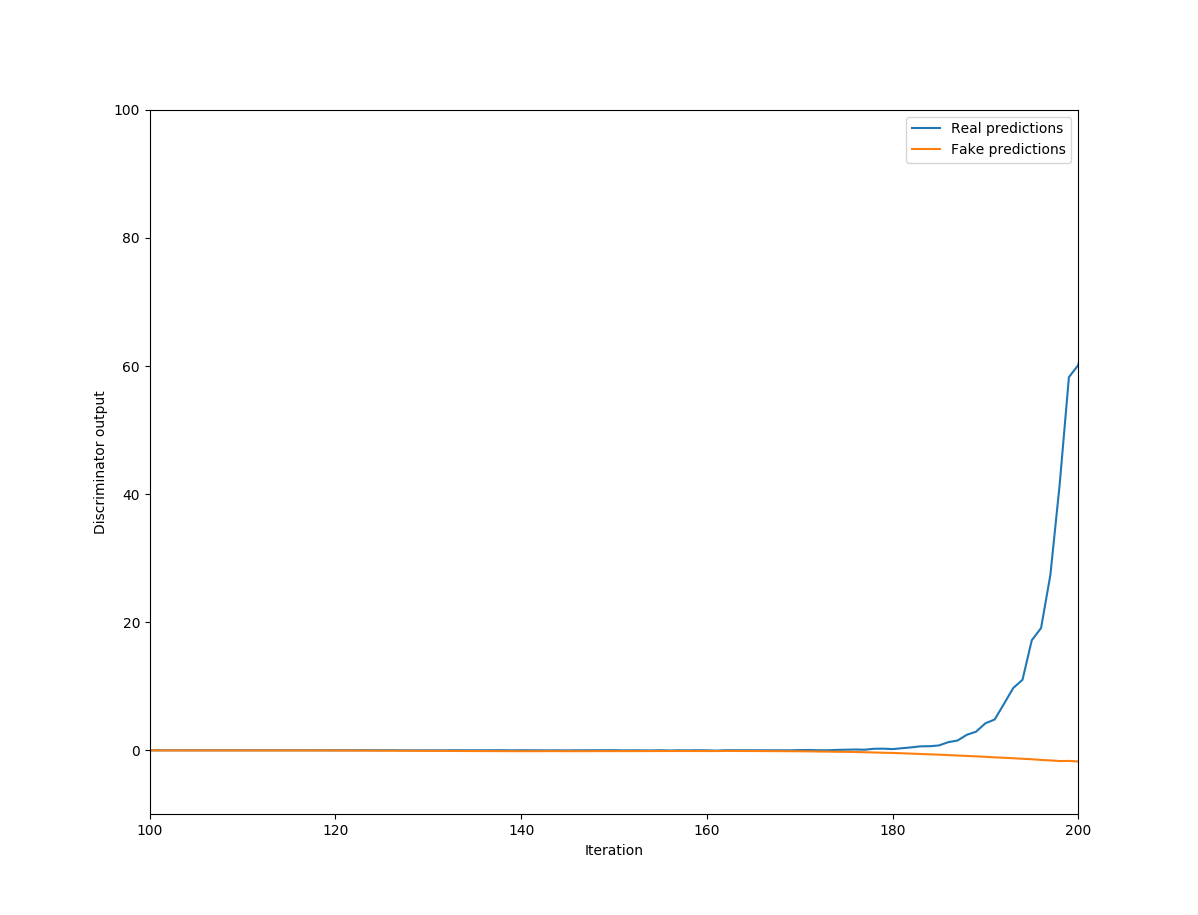
\includegraphics[width=\textwidth]{results/fadeInDG1.png}
%        \caption{Fade in new layers}
%        \label{fig:freezeInDG2}
%    \end{subfigure}
%    \caption{Discriminator output on real and fake images during transition between 16x16 and 32x32 resolution images for the different transition strategies.}
%    \label{fig:fadeVsFreeze}
%\end{figure}


\section{\acrlong{aegan}}
The final method tested in this project is based on a combination of autoencoders and \acrshort{gans}, named the \acrfull{aegan}. The proposed method consists of simultaneuously training a denoising autoencoder and a \acrshort{gan}, using the same network as generator and decoder. The idea is conceptually similar to the VAEGAN framework \parencite{LarsenSW15autoencodingbeyond}. There are two major differences between this method and the VAEGAN framework, first and foremost the autoencoder trained in this method is deterministic and trained with the mean squared error loss functions. Secondly, the adversarial loss is not used to train the autoencoder, instead a normal GAN is trained separately form the autoencoder but with the decoder network as the generator. 

Given enough capacity in the generator and encoder, the global minimum for the autoencoder training in this setting corresponds to the autoencoder learning the identity mapping. This causes the generator to generate realistic images on the points in the latent space the autoencoder maps the original data onto. The optimal generator in the \acrshort{gan} framework maps the entire latent space to realistic images. From this point of view the two objectives should lead to the same solution, however \acrshort{gans} tend to suffer from mode collapse and autoencoders often produce poor samples in terms of visual quality. Therefore if this method converges, it should enforce the decoded images to be sharp and the generator to capture the entire training data distribution.
% Idé till presentationen: "Variational autoencoders are stable and good at ...blablabla... . On the other hand there are two major problems with variational autoencoders, 1: they are variational (Åtgärda KL-term), 2: they are autoencoders (pixel-loss ersätts med GANs)."

\section{Training setup}
For the experiments, all models were trained using the Adamax optimizer \parencite{kingma2014adam} with $8$ samples per batch, a learning rate of $0.0001$, $\beta_1 = 0.5$ and $\beta_2 = 0.99$. The non-progressive models were trained for around 440000 iterations, however convergence of the methods might be either much faster or much slower than this depending on the model. The progressive training consisted of $100000$ iterations per stage, with $10000$ iterations of fade in between the stages.

